% Make listings font size smaller for input and output files
\lstset{basicstyle=\ttfamily\scriptsize, columns=fullflexible, keepspaces=true}
\section{Benchmarks}
The accuracy and robustness of the code is tested by solving some sample 
problems, the exact solutions of which were computed apriori via the classical
beam theory. The results are presented in this section using the following scheme: 
\begin{itemize}
    \item Demonstration of the problem
    \item Input file that addresses the problem
    \item Output file generated by the program after analysis
    \item Diagrams obtained by postprocessing 
    \item Comparison of the results of numerical and analytical solutions
\end{itemize}
Each problem considered in the first part comprise a single or continous beam 
subjected to  a certain external loading and set of restraints. The second part 
deals with a one-bay one-storey frame under different loads and support conditions.
Then some problems that involve more specialized cases of matrix structural analysis
are investigated, such as beams with shear deformability, elastic restraints and links and
thermal loadings. The fourth and final part is devoted to the analysis of prestressed beams.
\par
The error in the desired quantities for each numerical solution is presented by using the true
percent relative error according to the following definition:
\begin{equation*}
    \epsilon_{r,t} = \frac{|exact \: value - numerical \: value|}
                          {|exact \: value|} \times 100
\end{equation*}
%
% PART I: BEAM BENCHMARKS
%
\subsection{Single Beam Under Various Loading and Support Conditions}
%
% PROBLEM 1
%
\subsubsection{Problem 1: Simple Beam - Uniformly Distributed Load}
\begin{figure}[h]
    \includegraphics[scale=0.75]{%
                            bm_figures/turtle_figures/bm01_turtle.pdf}
    \centering
    \caption{Problem 1: Loading, geometry and supports}
    \label{fig:bm01_turtle}
\end{figure}
\lstinputlisting{input_files/bm01_input.dat}
\lstinputlisting{output_files/bm01_output.dat}
% Deformed
\begin{figure}[!htb]
    \includegraphics[width=\textwidth, keepaspectratio]{%
                     bm_figures/vtk_figures/bm01_deformed.pdf}
    \centering
    \caption{Problem 1, Deformed Shape}
    \label{fig:bm01_deformed}
\end{figure}
% Shear
\begin{figure}[!htb]
    \includegraphics[width=\textwidth, keepaspectratio]{%
                     bm_figures/vtk_figures/bm01_shear.pdf}
    \centering
    \caption{Problem 1, Shear Force Diagram}
    \label{fig:bm01_shear}
\end{figure}
% Moment
\begin{figure}[!htb]
    \includegraphics[width=\textwidth, keepaspectratio]{%
                     bm_figures/vtk_figures/bm01_moment.pdf}
    \centering
    \caption{Problem 1, Bending Moment Diagram}
    \label{fig:bm01_moment}
\end{figure}
% Error
\begin{table}[h!]
\centering
\begin{tabular}{ c| c c c c }
    & Exact Expression & Exact Value & Computed Value & \% RE \\ \hline \\
    V   & $\dfrac{\omega l}{2}$ &  0.12500E+03 & 0.12500E+03 & 0.0\% \\ \\
    $M_{max}$ & $\dfrac{\omega l^2}{8}$ &  0.31250E+03 & 0.31250E+03 & 0.0\% \\ \\
    $\delta_{max}$ & $\dfrac{5 \omega l^4}{384EI}$ & -0.63578E-02 & -0.63578E-02 & 0.0\% \\
\end{tabular}
\end{table}

%
% PROBLEM 5
%

\clearpage
\subsubsection{Problem 5: Simple Beam - Load Increasing Uniformly To One End}
\begin{figure}[h]
    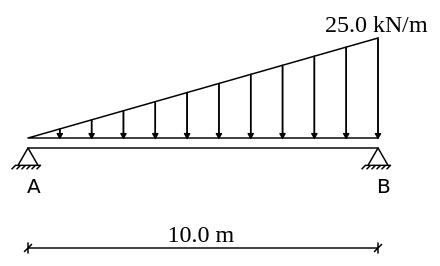
\includegraphics[scale=0.75]{%
                            bm_figures/turtle_figures/bm05_turtle.pdf}
    \centering
    \caption{Problem 5: Loading, geometry and supports}
    \label{fig:bm05_turtle}
\end{figure}
\lstinputlisting{input_files/bm05_input.dat}
\lstinputlisting{output_files/bm05_output.dat}
% Deformed
\begin{figure}[!htb]
    \includegraphics[width=\textwidth, keepaspectratio]{%
                     bm_figures/vtk_figures/bm05_deformed.pdf}
    \centering
    \caption{Problem 5, Deformed Shape}
    \label{fig:bm05_deformed}
\end{figure}
% Shear
\begin{figure}[!htb]
    \includegraphics[width=\textwidth, keepaspectratio]{%
                     bm_figures/vtk_figures/bm05_shear.pdf}
    \centering
    \caption{Problem 5, Shear Force Diagram}
    \label{fig:bm05_shear}
\end{figure}
% Moment
\begin{figure}[!htb]
    \includegraphics[width=\textwidth, keepaspectratio]{%
                     bm_figures/vtk_figures/bm05_moment.pdf}
    \centering
    \caption{Problem 5, Bending Moment Diagram}
    \label{fig:bm05_moment}
\end{figure}
% Error
\begin{table}[h!]
\centering
\begin{tabular}{ c| c c c c }
    & Exact Expression & Exact Value & Computed Value & \% RE \\ \hline \\
    $V_A$   & $\dfrac{\omega l}{6}$ &  0.41667E+02 & 0.41667E+02 & 0.0\% \\ \\
    $V_B$  & $\dfrac{ \omega l}{3}$ &  0.83333E+02 & 0.83333E+02 & 0.0\% \\ \\
    $M_{max}$ & $\dfrac{\omega l^2}{9\sqrt{3}}$ &  0.16037E+03 & 0.16037E+03 & 0.0\% \\ \\
\end{tabular}
\end{table}

%
% PROBLEM 6
%

\clearpage
\subsubsection{Problem 6: Simple Beam - Load Increasing Uniformly To Center}
\begin{figure}[h]
    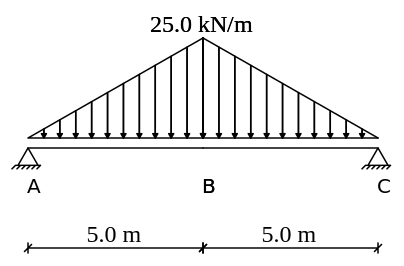
\includegraphics[scale=0.75]{%
                            bm_figures/turtle_figures/bm06_turtle.pdf}
    \centering
    \caption{Problem 6: Loading, geometry and supports}
    \label{fig:bm06_turtle}
\end{figure}
\lstinputlisting{input_files/bm06_input.dat}
\lstinputlisting{output_files/bm06_output.dat}
% Deformed
\begin{figure}[!htb]
    \includegraphics[width=\textwidth, keepaspectratio]{%
                     bm_figures/vtk_figures/bm06_deformed.pdf}
    \centering
    \caption{Problem 6, Deformed Shape}
    \label{fig:bm06_deformed}
\end{figure}
% Shear
\begin{figure}[!htb]
    \includegraphics[width=\textwidth, keepaspectratio]{%
                     bm_figures/vtk_figures/bm06_shear.pdf}
    \centering
    \caption{Problem 6, Shear Force Diagram}
    \label{fig:bm06_shear}
\end{figure}
% Moment
\begin{figure}[!htb]
    \includegraphics[width=\textwidth, keepaspectratio]{%
                     bm_figures/vtk_figures/bm06_moment.pdf}
    \centering
    \caption{Problem 6, Bending Moment Diagram}
    \label{fig:bm06_moment}
\end{figure}
% Error
\begin{table}[h!]
\centering
\begin{tabular}{ c| c c c c }
    & Exact Expression & Exact Value & Computed Value & \% RE \\ \hline \\
    V   & $\dfrac{\omega l}{4}$ &  0.62500E+02 & 0.62500E+02 & 0.0\% \\ \\
    $M_{max}$ & $\dfrac{\omega l^2}{12}$ & 0.20833E+03 & 0.20833E+03 & 0.0\% \\ \\
    $\delta_{max}$ & $\dfrac{\omega l^4}{120EI}$ & -0.40690E-02 & -0.40690E-02 & 0.0\% \\
\end{tabular}
\end{table}

%
% PROBLEM 9
%

\clearpage
\subsubsection{Problem 9: Simple Beam - Two Equal Concentrated Loads Symmetrically Placed}
\begin{figure}[h]
    \includegraphics[scale=0.75]{%
                            bm_figures/turtle_figures/bm09_turtle.pdf}
    \centering
    \caption{Problem 9: Loading, geometry and supports}
    \label{fig:bm09_turtle}
\end{figure}
\lstinputlisting{input_files/bm09_input.dat}
\lstinputlisting{output_files/bm09_output.dat}
% Deformed
\begin{figure}[!htb]
    \includegraphics[width=\textwidth, keepaspectratio]{%
                     bm_figures/vtk_figures/bm09_deformed.pdf}
    \centering
    \caption{Problem 9, Deformed Shape}
    \label{fig:bm09_deformed}
\end{figure}
% Shear
\begin{figure}[!htb]
    \includegraphics[width=\textwidth, keepaspectratio]{%
                     bm_figures/vtk_figures/bm09_shear.pdf}
    \centering
    \caption{Problem 9, Shear Force Diagram}
    \label{fig:bm09_shear}
\end{figure}
% Moment
\begin{figure}[!htb]
    \includegraphics[width=\textwidth, keepaspectratio]{%
                     bm_figures/vtk_figures/bm09_moment.pdf}
    \centering
    \caption{Problem 9, Bending Moment Diagram}
    \label{fig:bm09_moment}
\end{figure}
% Error
\begin{table}[h!]
\centering
\begin{tabular}{ c| c c c c }
    & Exact Expression & Exact Value & Computed Value & \% RE \\ \hline \\
    V   & P & 0.15000E+02 & 0.15000E+02 & 0.0\% \\ \\
    $M_{max}$ & Pa & 0.37500E+02 & 0.37500E+02 & 0.0\% \\ \\
    $\delta_{max}$ & $\dfrac{Pa}{24EI}(3l^2 - 4a^2)$ & -0.83923E-03 & -0.83923E-03 & 0.0\% \\
\end{tabular}
\end{table}

%
% PROBLEM 14
%

\clearpage
\subsubsection{Problem 14: Cantilever Beam - Concentrated Load At Any Point}
\begin{figure}[h]
    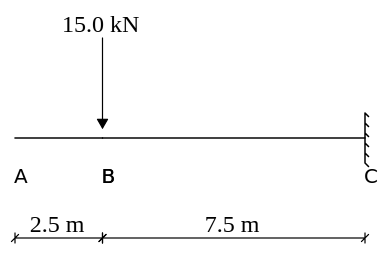
\includegraphics[scale=0.75]{%
                            bm_figures/turtle_figures/bm14_turtle.pdf}
    \centering
    \caption{Problem 14: Loading, geometry and supports}
    \label{fig:bm14_turtle}
\end{figure}
\lstinputlisting{input_files/bm14_input.dat}
\lstinputlisting{output_files/bm14_output.dat}
% Deformed
\begin{figure}[!htb]
    \includegraphics[width=\textwidth, keepaspectratio]{%
                     bm_figures/vtk_figures/bm14_deformed.pdf}
    \centering
    \caption{Problem 14, Deformed Shape}
    \label{fig:bm14_deformed}
\end{figure}
% Shear
\begin{figure}[!htb]
    \includegraphics[width=\textwidth, keepaspectratio]{%
                     bm_figures/vtk_figures/bm14_shear.pdf}
    \centering
    \caption{Problem 14, Shear Force Diagram}
    \label{fig:bm14_shear}
\end{figure}
% Moment
\begin{figure}[!htb]
    \includegraphics[width=\textwidth, keepaspectratio]{%
                     bm_figures/vtk_figures/bm14_moment.pdf}
    \centering
    \caption{Problem 14, Bending Moment Diagram}
    \label{fig:bm14_moment}
\end{figure}
% Error
\begin{table}[h!]
\centering
\begin{tabular}{ c| c c c c }
    & Exact Expression & Exact Value & Computed Value & \% RE \\ \hline \\
    V   & P & 0.15000E+02 & 0.15000E+02 & 0.0\% \\ \\
    $M_{max}$ & Pb & 0.11250E+03 & 0.11250E+03 & 0.0\% \\ \\
    $\delta_{max}$ & $\dfrac{Pb^2}{6EI}(3l-b)$ & -0.61798E-02 & -0.61798E-02 & 0.0\% \\
    $\delta_{B}$ & $\dfrac{Pb^3}{3EI}$ & -0.41199E-02 & -0.41199E-02 & 0.0\% \\
\end{tabular}
\end{table}

%
% PROBLEM 15
%

\clearpage
\subsubsection{Problem 15: Beam Fixed at One End, Supported at Other - Uniformly Distributed Load}
\begin{figure}[h]
    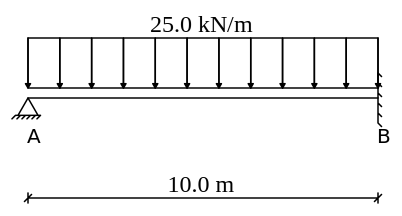
\includegraphics[scale=0.75]{%
                            bm_figures/turtle_figures/bm15_turtle.pdf}
    \centering
    \caption{Problem 15: Loading, geometry and supports}
    \label{fig:bm15_turtle}
\end{figure}
\lstinputlisting{input_files/bm15_input.dat}
\lstinputlisting{output_files/bm15_output.dat}
% Deformed
\begin{figure}[!htb]
    \includegraphics[width=\textwidth, keepaspectratio]{%
                     bm_figures/vtk_figures/bm15_deformed.pdf}
    \centering
    \caption{Problem 15, Deformed Shape}
    \label{fig:bm15_deformed}
\end{figure}
% Shear
\begin{figure}[!htb]
    \includegraphics[width=\textwidth, keepaspectratio]{%
                     bm_figures/vtk_figures/bm15_shear.pdf}
    \centering
    \caption{Problem 15, Shear Force Diagram}
    \label{fig:bm15_shear}
\end{figure}
% Moment
\begin{figure}[!htb]
    \includegraphics[width=\textwidth, keepaspectratio]{%
                     bm_figures/vtk_figures/bm15_moment.pdf}
    \centering
    \caption{Problem 15, Bending Moment Diagram}
    \label{fig:bm15_moment}
\end{figure}
% Error
\begin{table}[h!]
\centering
\begin{tabular}{ c| c c c c }
    & Exact Expression & Exact Value & Computed Value & \% RE \\ \hline \\
    $V_A$  & $\dfrac{3\omega l}{8}$ & 0.93750E+02 & 0.93750E+02 & 0.0\% \\ \\
    $V_B$  & $\dfrac{5\omega l}{8}$ & 0.15625E+03 & 0.15625E+03 & 0.0\% \\ \\
    $M_{max}^-$ & $\dfrac{\omega l^2}{8}$ & 0.31250E+03 & 0.31250E+03 & 0.0\% \\ \\
    $M_{max}^+$ & $\dfrac{9\omega l^2}{128}$ & 0.17578E+03 & 0.17576E+03 & 0.014\% \\ \\
    $\delta_{max}$ & $\dfrac{\omega l^4}{185EI}$ & -0.26394E-02 & -0.26446E-02 & 0.197\% \\
\end{tabular}
\end{table}

%
% PROBLEM 19
%

\clearpage
\subsubsection{Problem 19: Beam Overhanging One Support - Uniformly Distributed Load on Overhang}
\begin{figure}[h]
    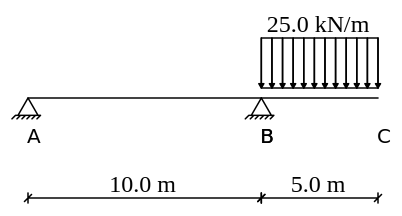
\includegraphics[scale=0.75]{%
                            bm_figures/turtle_figures/bm19_turtle.pdf}
    \centering
    \caption{Problem 19: Loading, geometry and supports}
    \label{fig:bm19_turtle}
\end{figure}
\lstinputlisting{input_files/bm19_input.dat}
\lstinputlisting{output_files/bm19_output.dat}
% Deformed
\begin{figure}[!htb]
    \includegraphics[width=\textwidth, keepaspectratio]{%
                     bm_figures/vtk_figures/bm19_deformed.pdf}
    \centering
    \caption{Problem 19, Deformed Shape}
    \label{fig:bm19_deformed}
\end{figure}
% Shear
\begin{figure}[!htb]
    \includegraphics[width=\textwidth, keepaspectratio]{%
                     bm_figures/vtk_figures/bm19_shear.pdf}
    \centering
    \caption{Problem 19, Shear Force Diagram}
    \label{fig:bm19_shear}
\end{figure}
% Moment
\begin{figure}[!htb]
    \includegraphics[width=\textwidth, keepaspectratio]{%
                     bm_figures/vtk_figures/bm19_moment.pdf}
    \centering
    \caption{Problem 19, Bending Moment Diagram}
    \label{fig:bm19_moment}
\end{figure}
% Error
\begin{table}[h!]
\centering
\begin{tabular}{ c| c c c c }
    & Exact Expression & Exact Value & Computed Value & \% RE \\ \hline \\
    $V_A$  & $\dfrac{\omega a^2}{2l}$ & 0.31250E+02 & 0.31250E+02 & 0.0\% \\ \\
    $V_B$  & $\omega a$ & 0.12500E+03 & 0.12500E+03 & 0.0\% \\ \\
    $M_{max}$ & $\dfrac{\omega a^2}{2}$ & 0.31250E+03 & 0.31250E+03 & 0.0\% \\ \\
    $\delta_{max}$ & $\dfrac{\omega a^3}{24EI}(4l+3a)$ & -0.13987E-01 &-0.13987E-01 & 0.0\% \\
\end{tabular}
\end{table}

%
% PROBLEM 24
%

\clearpage
\subsubsection{Problem 24: Beam Fixed at Both Ends - Concentrated Load at Center}
\begin{figure}[h]
    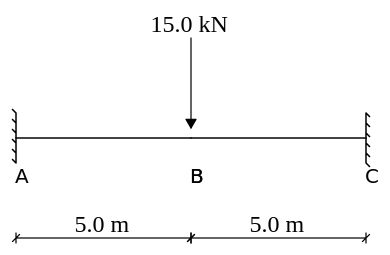
\includegraphics[scale=0.75]{%
                            bm_figures/turtle_figures/bm24_turtle.pdf}
    \centering
    \caption{Problem 24: Loading, geometry and supports}
    \label{fig:bm24_turtle}
\end{figure}
\lstinputlisting{input_files/bm24_input.dat}
\lstinputlisting{output_files/bm24_output.dat}
% Deformed
\begin{figure}[!htb]
    \includegraphics[width=\textwidth, keepaspectratio]{%
                     bm_figures/vtk_figures/bm24_deformed.pdf}
    \centering
    \caption{Problem 24, Deformed Shape}
    \label{fig:bm24_deformed}
\end{figure}
% Shear
\begin{figure}[!htb]
    \includegraphics[width=\textwidth, keepaspectratio]{%
                     bm_figures/vtk_figures/bm24_shear.pdf}
    \centering
    \caption{Problem 24, Shear Force Diagram}
    \label{fig:bm24_shear}
\end{figure}
% Moment
\begin{figure}[!htb]
    \includegraphics[width=\textwidth, keepaspectratio]{%
                     bm_figures/vtk_figures/bm24_moment.pdf}
    \centering
    \caption{Problem 24, Bending Moment Diagram}
    \label{fig:bm24_moment}
\end{figure}
% Error
\begin{table}[h!]
\centering
\begin{tabular}{ c| c c c c }
    & Exact Expression & Exact Value & Computed Value & \% RE \\ \hline \\
    V  & $\dfrac{P}{2}$ & 0.75000E+01 & 0.75000E+01 & 0.0\% \\ \\
    $M_{max}$ & $\dfrac{Pl}{8}$ & 0.18750E+02 & 0.18750E+02 & 0.0\% \\ \\
    $\delta_{max}$ & $\dfrac{Pl^3}{192EI}$ & -0.15259E-03 & -0.15259E-03 & 0.0\% \\
\end{tabular}
\end{table}

%
% PROBLEM 27
%

\clearpage
\subsubsection{Problem 27: Continuous Beam - Two Equal Spans - Concentrated Load At Center of One Span}
\begin{figure}[h]
    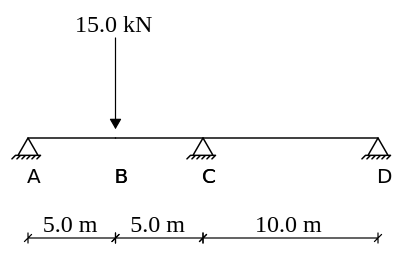
\includegraphics[scale=0.75]{%
                            bm_figures/turtle_figures/bm27_turtle.pdf}
    \centering
    \caption{Problem 27: Loading, geometry and supports}
    \label{fig:bm27_turtle}
\end{figure}
\lstinputlisting{input_files/bm27_input.dat}
\lstinputlisting{output_files/bm27_output.dat}
% Deformed
\begin{figure}[!htb]
    \includegraphics[width=\textwidth, keepaspectratio]{%
                     bm_figures/vtk_figures/bm27_deformed.pdf}
    \centering
    \caption{Problem 27, Deformed Shape}
    \label{fig:bm27_deformed}
\end{figure}
% Shear
\begin{figure}[!htb]
    \includegraphics[width=\textwidth, keepaspectratio]{%
                     bm_figures/vtk_figures/bm27_shear.pdf}
    \centering
    \caption{Problem 27, Shear Force Diagram}
    \label{fig:bm27_shear}
\end{figure}
% Moment
\begin{figure}[!htb]
    \includegraphics[width=\textwidth, keepaspectratio]{%
                     bm_figures/vtk_figures/bm27_moment.pdf}
    \centering
    \caption{Problem 27, Bending Moment Diagram}
    \label{fig:bm27_moment}
\end{figure}
% Error
\begin{table}[h!]
\centering
\begin{tabular}{ c| c c c c }
    & Exact Expression & Exact Value & Computed Value & \% RE \\ \hline \\
    $V_A$  & $\dfrac{13}{32}P$ & 0.60938E+01 & 0.60938E+01 & 0.0\% \\ \\
    $V_C$  & $\dfrac{19}{32}P$ & 0.89062E+01 & 0.89062E+01 & 0.0\% \\ \\
    $V_D$  & $\dfrac{3}{32}P$ & 0.14062E+01 & 0.14062E+01 & 0.0\% \\ \\
    $M_C$ & $\dfrac{3}{32}Pl$ & 0.14062E+02 & 0.14062E+02 & 0.0\% \\ \\
    $M_{max}$ & $\dfrac{13}{64}Pl$ & 0.30469E+02 & 0.30469E+02 & 0.0\% \\ \\
\end{tabular}
\end{table}

%
% PROBLEM 29
%

\clearpage
\subsubsection{Problem 29: Continuous Beam - Two Equal Spans - Uniformly Distributed Load}
\begin{figure}[h]
    \includegraphics[scale=0.75]{%
                            bm_figures/turtle_figures/bm29_turtle.pdf}
    \centering
    \caption{Problem 29: Loading, geometry and supports}
    \label{fig:bm29_turtle}
\end{figure}
\lstinputlisting{input_files/bm29_input.dat}
\lstinputlisting{output_files/bm29_output.dat}
% Deformed
\begin{figure}[!htb]
    \includegraphics[width=\textwidth, keepaspectratio]{%
                     bm_figures/vtk_figures/bm29_deformed.pdf}
    \centering
    \caption{Problem 29, Deformed Shape}
    \label{fig:bm29_deformed}
\end{figure}
% Shear
\begin{figure}[!htb]
    \includegraphics[width=\textwidth, keepaspectratio]{%
                     bm_figures/vtk_figures/bm29_shear.pdf}
    \centering
    \caption{Problem 29, Shear Force Diagram}
    \label{fig:bm29_shear}
\end{figure}
% Moment
\begin{figure}[!htb]
    \includegraphics[width=\textwidth, keepaspectratio]{%
                     bm_figures/vtk_figures/bm29_moment.pdf}
    \centering
    \caption{Problem 29, Bending Moment Diagram}
    \label{fig:bm29_moment}
\end{figure}
% Error
\begin{table}[h!]
\centering
\begin{tabular}{ c| c c c c }
    & Exact Expression & Exact Value & Computed Value & \% RE \\ \hline \\
    $V_A$  & $\dfrac{3\omega l}{8}$ & 0.93750E+02 & 0.93750E+02 & 0.0\% \\ \\
    $V_B$  & $\dfrac{5\omega l}{8}$ & 0.15625E+03 & 0.15625E+03 & 0.0\% \\ \\
    $M_{max}^+$ & $\dfrac{9 \omega l^2}{128}$ & 0.17578E+03 & 0.17578E+03 & 0.0\% \\ \\
    $M_{max}^-$ & $\dfrac{\omega l^2}{8}$ & 0.31250E+03 & 0.31250E+03 & 0.0\% \\ \\
    $\delta_{max}$ & $\dfrac{\omega l^4}{185EI}$ & -0.26394E-02 & -0.26336E-03 & 0.220\% \\
\end{tabular}
\end{table}

